\documentclass[11pt]{article}
\usepackage[margin=1in]{geometry}
\usepackage{graphicx}
\usepackage{hyperref}
\begin{document}

\title{Automating information extraction from documents}
\maketitle


\noindent \textbf{\textit{Nobody said it was easy \\
No one ever said it would be this hard \\ \\}
}
\noindent Truer words haven't been spoken (or sang really) when it comes to extracting data from piles and piles of documents. As much as we like to believe otherwise, an enormous number of company transactions still involve paper work instead of digital means. Accountants and finance departments understand the pain and are desperately looking for an end-to-end solution which automates and digitalises the accounting workflows.  Book-keepers spend long hours on manual data entry from invoices, receipts and other documents costing meaningless effort, money and time. Good grief! why are still struggling to find a reliable solution that can put an end to this everlasting drain of resources. The complexity of automating this problem revolves around the variability of documents' format and structure. An invoice or a receipt can be created in millions of different styles which makes it impossible to take a 'template' based approach or 'fingerprinting' to sound fancier. Adding to the misery, reading text via traditional OCR (optical character recognition) is enigmatic and prone to error because it largely depends on the picture quality, shadows, and perspective from where the picture was captured. Enter the new kid on the block, Staple AI,  which uses computer vision and machine learning to imitate the human approach to extract the information from the semi-structured documents. \\

\noindent So Staple AI imitates human behaviour but why exactly? After all, they make errors, are really slow, and they demand (lots of) money. However, they are pretty good when it comes to finding information on a piece of paper just through a short glimpse.  For a document such as an invoice, a human doesn't need to read the entire text to understand and pick out the key-field values. Instead, they look for the structural and contextual cues, the general layout, and the formatting of the text. For example, it's fairly easy for a human to extract the 'Invoice number' or the 'Total amount' in the image below. No where in the image is it written: 'The invoice number is WN201901002' but we all understand it almost instantaneously. But why exactly is it so simple ? Is it the text in bold with the number on the right? Or is it the assignment via a colon that assigns a number to the word 'invoice number'? Probably the structure and the localisation of the text (as compared to a big paragraph like this) in a certain way helps. For machines, semi-structured information like this is difficult to interpret with traditional NLP (Natural Language Processing) tools because mostly there is no grammar or proper sentences involved which can correlate a value to field. So indeed copying a human sounds great!  \\

\begin{figure}
\centering
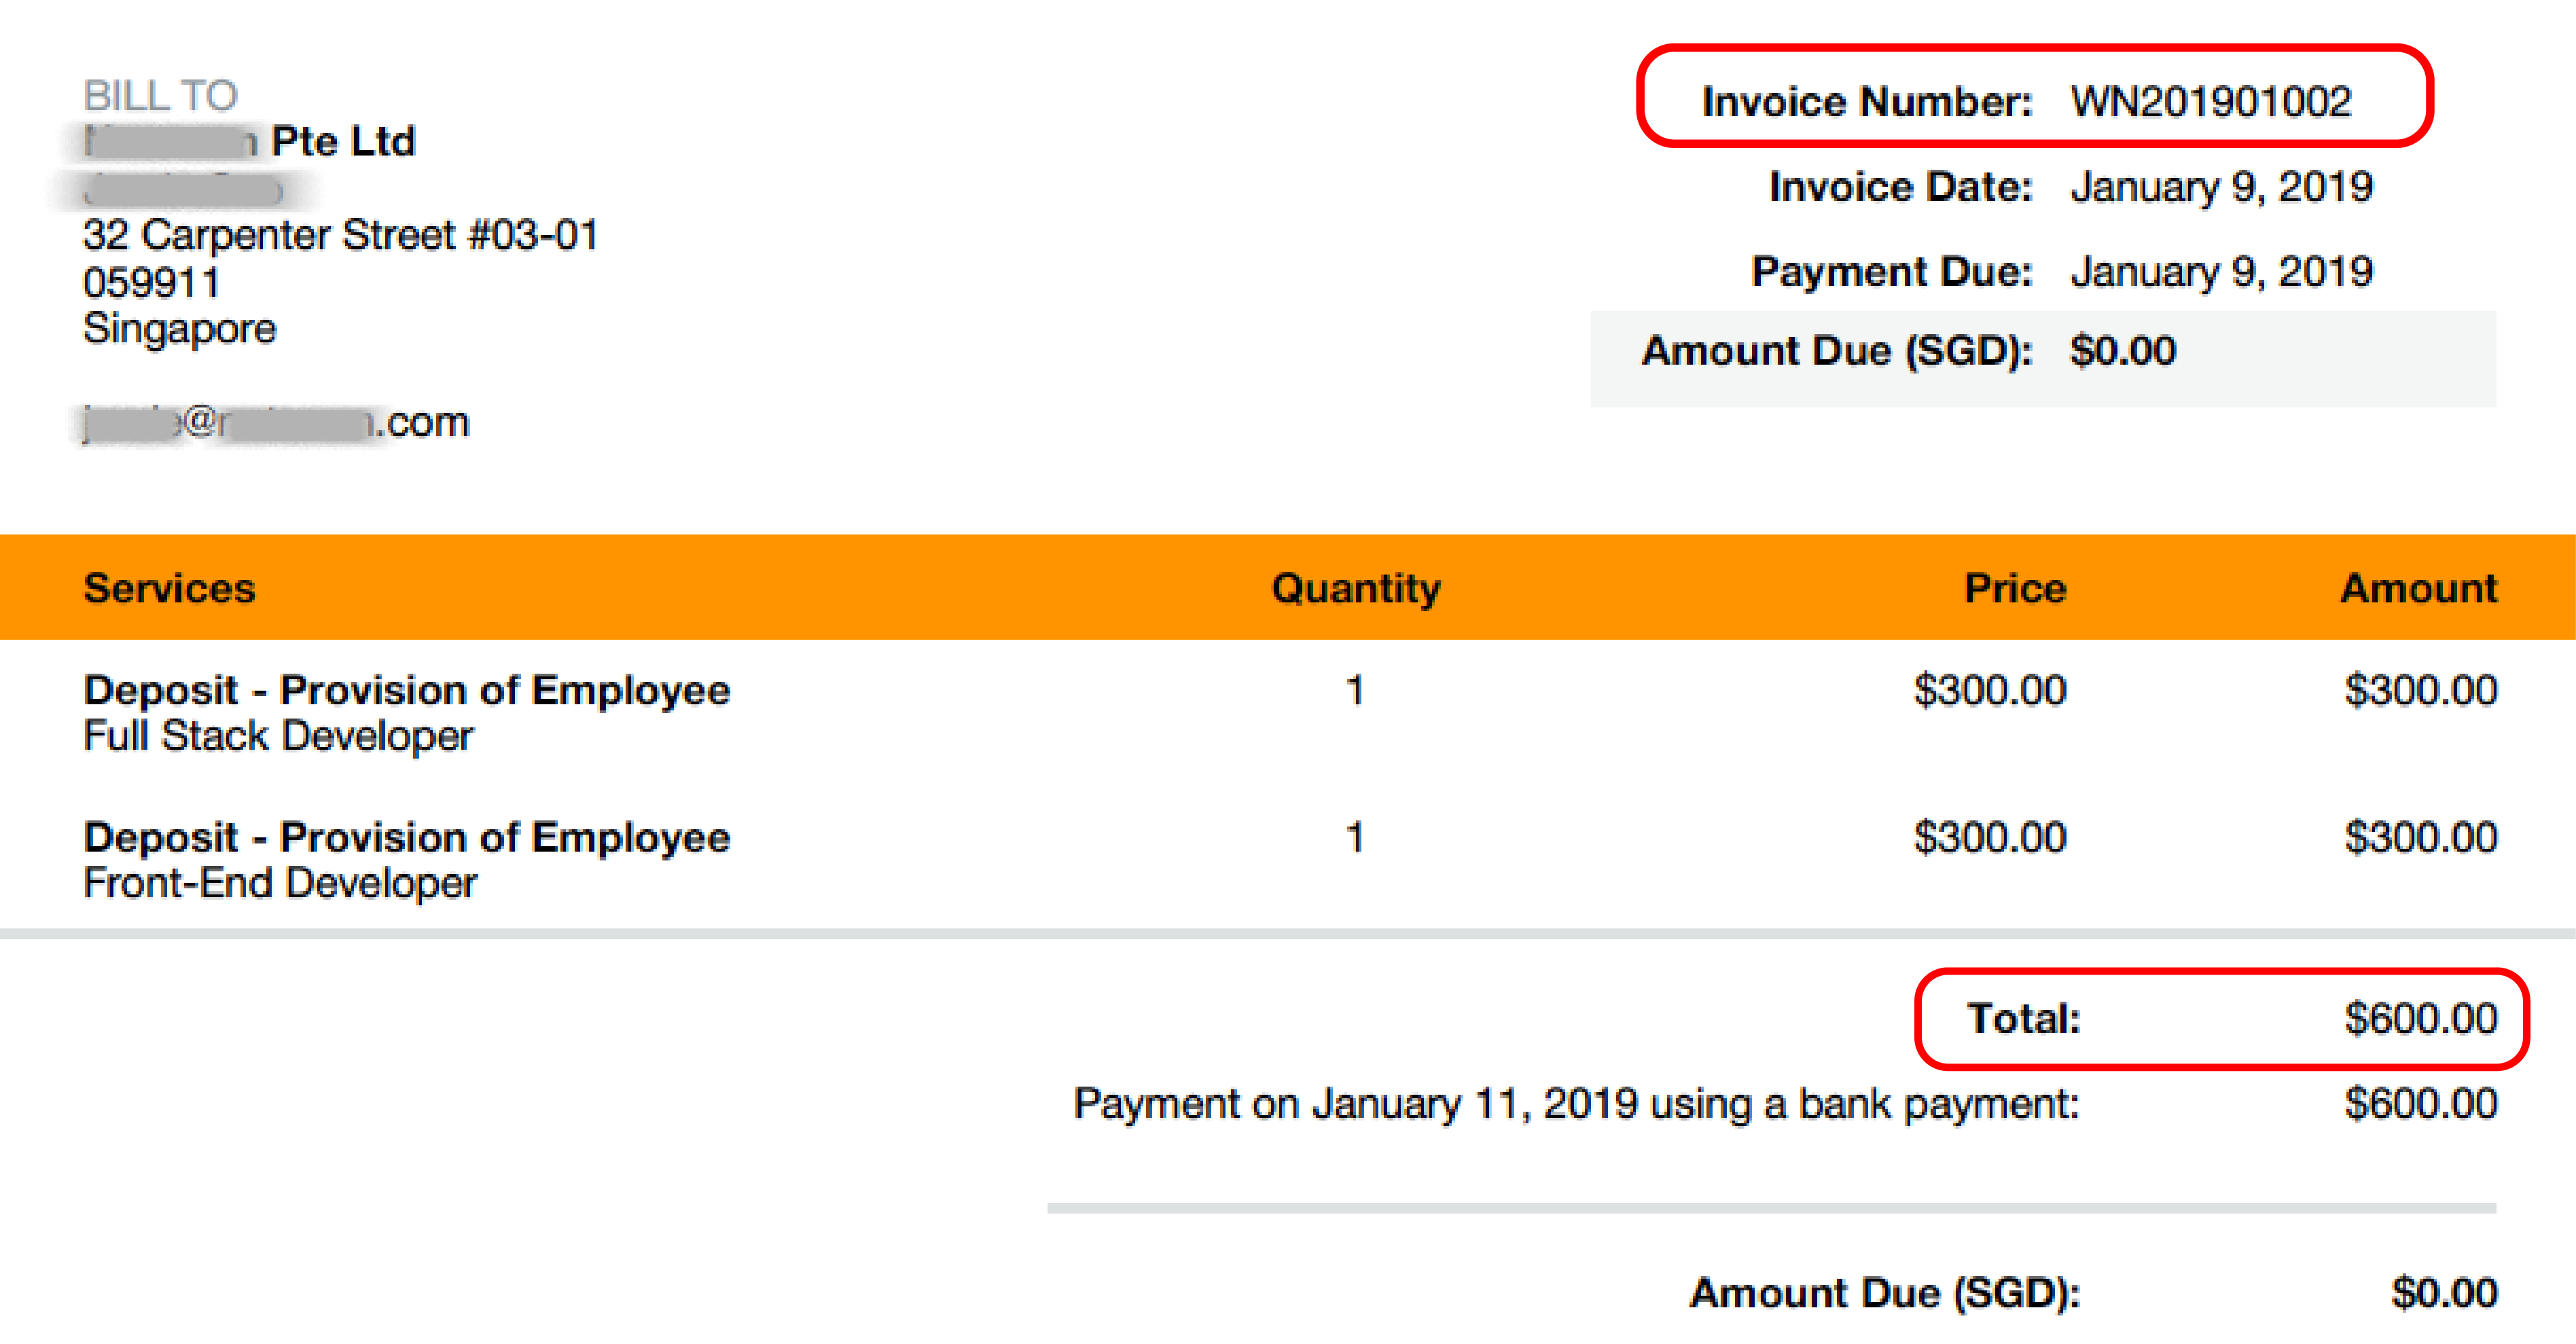
\includegraphics[scale= 0.4]{formatting}
\end{figure}


\noindent Staple extracts meaningful information from documents such as invoices, receipts, and purchase orders and transfers the digital data directly to your integrated accounting software or just to you in a clean JSON format (if that's what you are into). The Staple platform hunts for the key-information required for scanning the document such as the supplier's name, tax, total amount, invoice number, and most importantly, the line-items. The document can be in a pdf or an image format. For pdfs, the text is unskewed, dewarped, and without any washed off ink which makes life easier. Images are rather tricky because people are lazy and not everyone has the photography skills of a sixteen year old. Other problems such as shadows, local curling of the paper and washed off ink are extremely common. Thankfully there are sophisticated computer vision tools available that can get rid of the messy background and dewarp the picture. \\

\noindent In the first step, Staple cleans the image and prepares it for an optimal text detection to attain high reading accuracy. In the second step, the processed image is passed through an OCR engine where the text is extracted conserving the spatial information of the text on the page. After all, that's exactly how a human understands the context with the help of the structure and location of the text. After text detection, Staple's document scanning platform runs the detected text and its spatial information on the page through its proprietary model and outputs  a JSON file with the required fields and their values, the confidence of the values found, and the bounding box of the value with respect to the top left corner of the page. Staple understands that every document is beautiful and unique in its own way (just like every human) and no 'template' based society can contain their beauty. Staple celebrates this uniqueness and has built the invoice scanning platform such that it is capable of scanning documents independent of their structure, layout and design. \\

\noindent To visualise the capability of Staple's document scanning platform, Staple has built a free API and a \href{https://demo.staple.io/}{live demo} which can be used to scan documents such as invoices and receipts. At the moment, pdfs and images of invoices and receipts are accepted. The API is deployed via Amazon web services using Elastic beanstalk which dockerises the Flask application. Elastic Beanstalk maintains the deployment, manages the load and auto-scales with the help of a load balancer. The auto-scaling and load-capacity varies from 1 to 100,000 documents being scanned in a day. One can use the API separately or have Staple integrate your Xero accounting software where your details of the document would automatically be posted. Moreover, Staple has built a \href{https://reconciler.io/}{Reconciler} to further make the life of accountants easier by reconciling payments via Stripe. Enough said! Is it any good? Let's find out!


 \begin{figure}[h]
\centering
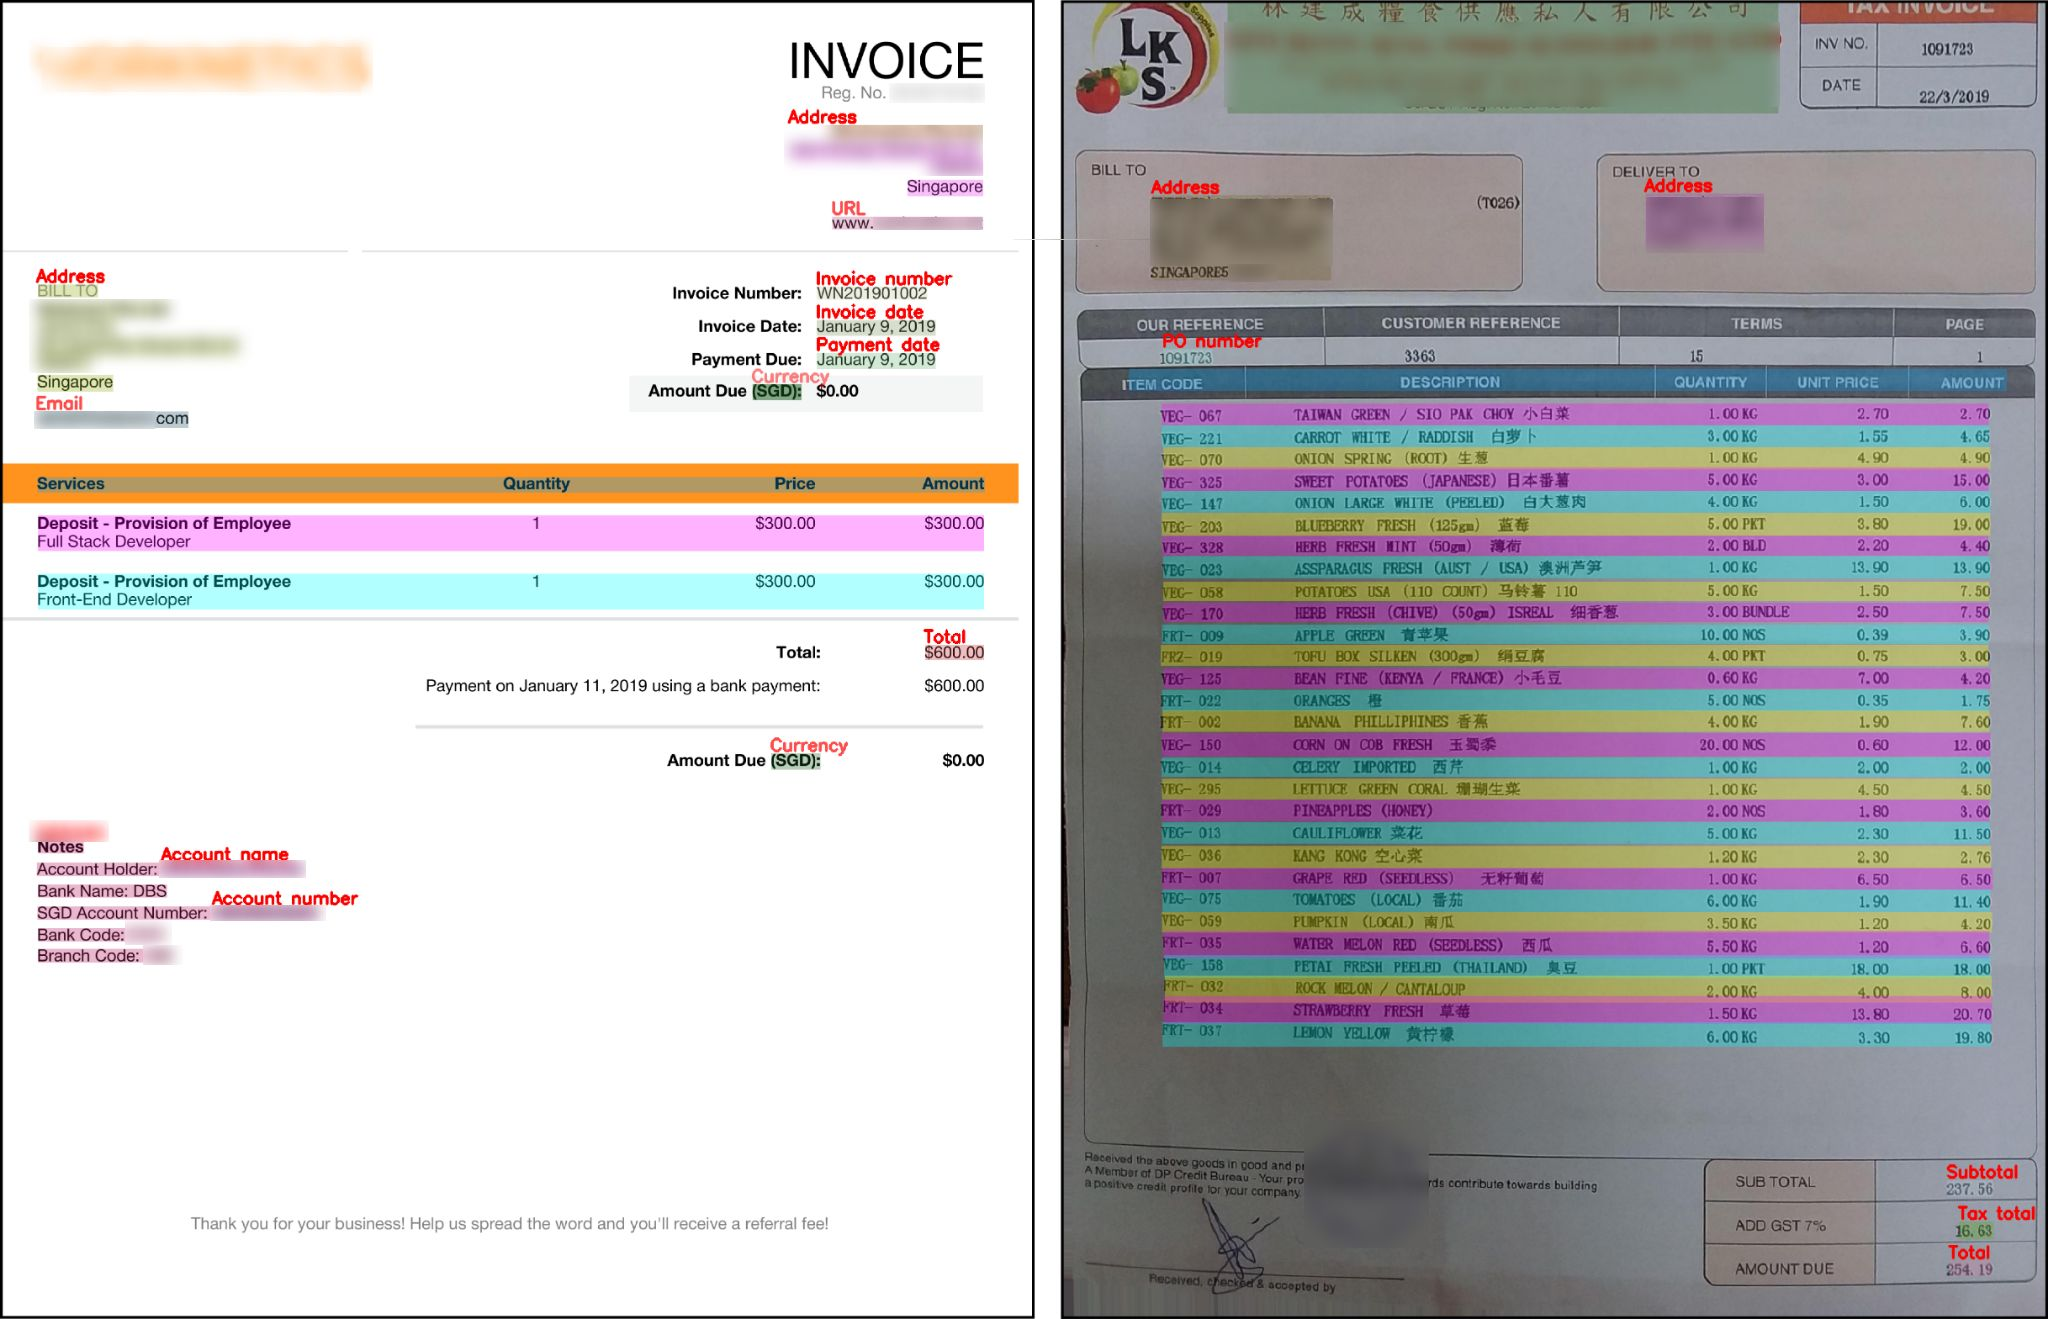
\includegraphics[scale= 0.22]{sample_i}

\label{default}
\end{figure}

 \begin{figure}[h]
\centering
\includegraphics[scale= 0.22]{sample_r}

\label{default}
\end{figure}


\noindent So let's free humans from all the mundane accounting tasks and leave them alone to what they do best, netflix and chill! 







 


\end{document}
